% format the chapter/section details
\chapter{Data and Methods}
\label{chap:data_methods}

% insert your text below the line
%-------------------------------------------
This research analyzes mobile scanning DWL data from various deployments from 2017 through 2023. Instrumentation details, data collection strategies, and quality-control and post processing techniques will be provided in this section. In total, 36 supercells were observed over 50 deployments with co-located radiosondes launched throughout operating periods (Fig. \ref{fig:dep_details}). 

\begin{figure}[h!]
    \centering
    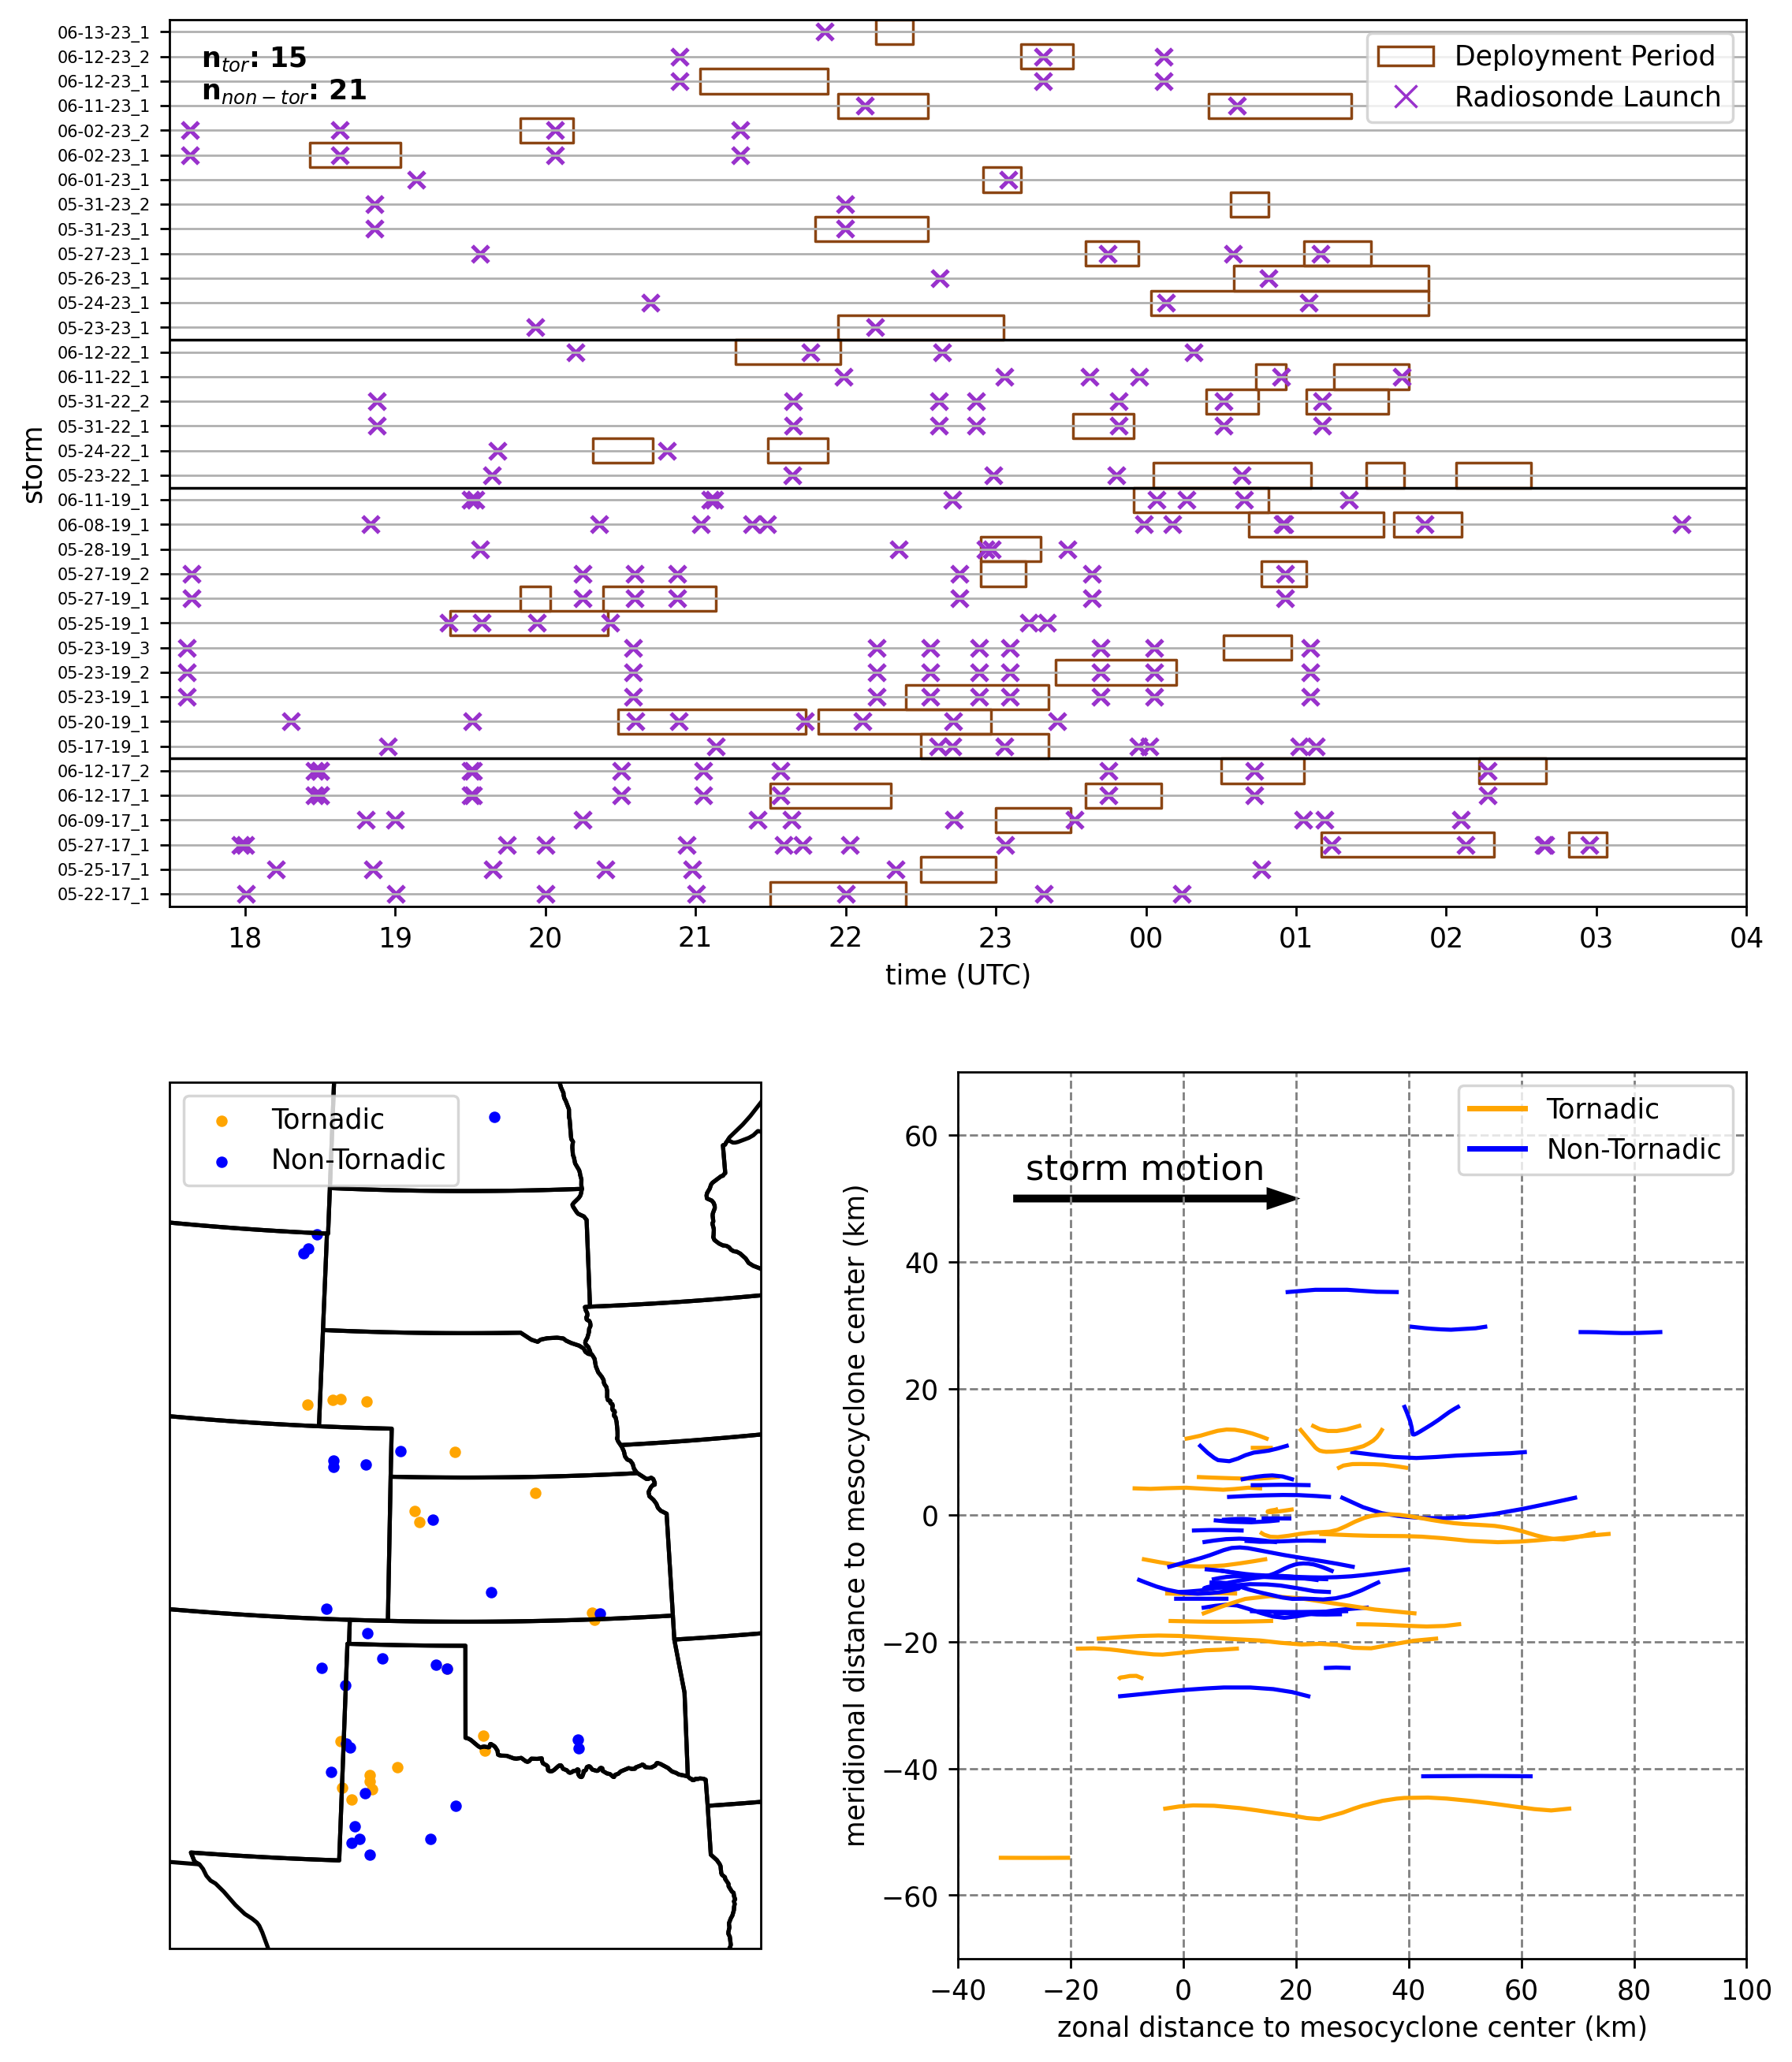
\includegraphics[width = 1\textwidth]{figures/dep_details.png}
    \caption{Timing of DWL deployments (blue rectangles) and co-located radiosonde launches (red marker) for each storm analyzed in this study (left). Deployment locations separated by tornadic (red) and non-tornadic (blue) storms (right).}
    \label{fig:dep_details}
\end{figure}

\section{Surface Observations}
In 2017, the National Severe Storms Laboratory (NSSL) deployed a DWL as part of their Collaborative Lower Atmospheric Mobile Profiling System - CLAMPS. This system was outfitted with a Vaisala met station which collected surface observations valid approximately 1 meter above the trailer (approximately 5 meters above ground level). Surface observations were logged every 5 seconds with an accuracy of $\pm$0.1$m\, s^{-1}$ in wind speed observations and $\pm$2$^\circ$ in wind direction \citep{WINDCAP}. 

From 2019 to 2023, the NSSL operated a DWL (two DWLs in 2022) from the bed of a Ford pickup truck. Mounted on this truck was a mobile mesonet rack where an RM Young 05103 Wind Monitor was used to collect surface horizontal wind speed and direction information every 1 second. These observations have wind speed accuracy within $\pm$0.3$m\, s^{-1}$ and wind direction accuracy within $\pm$3$^\circ$ \citep{waugh2021u}. Collected surface observations were used to subjectively determine the passage of various boundaries indicative of no longer sampling inflow air (e.g., a gust front passage).